\documentclass[12pt]{article}

\usepackage{graphicx}
\usepackage{paralist}
\usepackage{amsfonts}
\usepackage{listings}
\usepackage{hyperref}
\usepackage{tabto}

\hypersetup{colorlinks=true,
    linkcolor=blue,
    citecolor=blue,
    filecolor=blue,
    urlcolor=blue,
    unicode=false}

\oddsidemargin 0mm
\evensidemargin 0mm
\textwidth 160mm
\textheight 200mm

\pagestyle {plain}
\pagenumbering{arabic}
\usepackage{titlesec}

\setcounter{secnumdepth}{4}

\titleformat{\paragraph}
{\normalfont\normalsize\bfseries}{\theparagraph}{1em}{}
\titlespacing*{\paragraph}
{0pt}{3.25ex plus 1ex minus .2ex}{1.5ex plus .2ex}

\usepackage{fancyhdr}
\usepackage{fancyhdr}
\fancyhead[L]{\today\ }
\fancyhead[C]{SE 3XA3: SRS Rev 1}
\fancyhead[R]{Group 2: Genzter}
\pagestyle{fancy}

\title{Software Requirements Specification: Revision 1}
\author{Group 2 - Genzter \\
		\\ Binu, Amit - binua - 400023175
		\\ Bengezi, Mohamed - bengezim - 400021279
		\\ Samarasinghe, Sachin - samarya - 001430998
		\\ \today\
		\\Professor: Dr. Bokhari
		\\ Lab: L01}

\begin {document}
\maketitle

\newpage

{\centering
  \tableofcontents\par
}
\addtocontents{toc}{\protect\vspace{2.5em}}

\listoftables
\listoffigures
\newpage

\section{Revision History}
\begin{table}[h]
\begin{center}
\begin{tabular}{ | c | c | c | c | }
\hline
 Date & Version & Description & Author \\ 
\hline
 05/OCT/17 & 0.0 & Created SRS & Mohamed Bengezi, Amit Binu, \\  
&&&  Sachin Samarasinghe \\
\hline
  26/NOV/17 & 1.0 & Modified Requirements & Mohamed Bengezi, Amit Binu, \\
&&&  Sachin Samarasinghe \\
\hline
  01/DEC/17 & 1.0 & Updated terminology, requirements & Mohamed Bengezi, Amit Binu, \\
  &&and added figure(s) & Sachin Samarasinghe \\
\hline 
 & & & \\ 
\hline 
\end{tabular}
\end{center}
\caption{Revision History}
\end{table}
***Please Note, all updated material is written in \textcolor{blue}{blue}
\newpage
\section{Project Drivers}
\subsection{Purpose}
\tab This project addresses a very tedious and time-consuming issue that affects thousands of university students every year. When it comes to course selection, finding the perfect schedule is no easy feat. Various obstacles contribute to this difficulty, whether it be a core, lecture or tutorial conflicting with something else, or a certain course can only be taken in a certain semester, etc. The Timetable Generator solves this issue by taking a list of required courses as input, and outputting a set of viable schedules as output, allowing the user to select the most appealing option. The goal of this project is to successfully accomplish this in an efficient manner, with an easy-to-use interface.

\subsection{Stakeholders}
There are a couple of stakeholders for this project, including the Genzter team, and obviously the students of McMaster University. In this case, the client and customer are the same: the student body. As for the motivation, seeing as we are students, we have first hand experience with regards to what is expected, and what an acceptable project entails.

\subsection{Scope}
The scope of this project includes understanding McMaster University's course layout, course selection process, as well as how courses differ throughout the various fields of study at McMaster. Also within the scope is the behaviour of students, and how they prefer timetables, whether they generally prefer early classes, late classes, Friday's off, etc. 

\subsection{Constraints}
\begin{itemize}
  \item The project must at least re-implement all of the functionalities of the original software.
  \item Core functionalities must be completed by October 16 for the proof of concept demonstration.
  \item The back-end server must use HTTP to communicate with the client.
  \item When a valid timetable cannot be generated, the server must communicate that fact to the client.
  \item The server must be able to serve multiple clients concurrently.
  \item The server must keep each session isolated from other sessions.
\end{itemize}

\subsection{Naming Conventions}
At the moment there are no special naming conventions.

\subsection{Terminology}
\textcolor{blue}{It is assumed that the client or individual using this document understands basic web development terminology, such as Node.js or HTTP}
\begin{itemize}
  \item \textbf{Server} is the backend server powered by Node.js. This server manages sessions, calculates timetables and delivers the results to the client. The server uses HTTP to communicate with the client.
  
  \item \textbf{Client} refers to the web-based client side software that takes the user input and sends it to the server. Through the client, the users can choose the courses that they are interested in adding to their timetables. The client is programmed using HTML, CSS and Javascript.
  
  \item \textbf{Site} refers to the website that hosts the client. The users can access the application though the site.
  
  \item A \textbf{Session} refers to a visit of a user to the site. A session begins when the user's web browser connects to the site. And a session ends when the tab or the window that has the site opened is closed. During a session, a user can add, remove and generate a timetable for their selected courses.
  
  \item \textbf{Selected course list} is a list of courses that are selected by a specific user in the client. When commanded by the user, the client will submit the selected course list to the server and will wait for a response from the server.
  
  \item A \textbf{valid timetable} is a timetable for all the selected courses without any timing conflicts. This includes times and durations of lectures, tutorials and labs.
  
  \item \textbf{Scheduler} is the software module that is responsible for generating the timetables.
  
  \item \textbf{Scheduling algorithm} is the specific timetable generation algorithm used by the scheduler to generate timetables.
\end{itemize}

\newpage

\subsection{\textcolor{blue}{Functional Requirements}}

\subsubsection{Startup and User Input}
\begin{enumerate}
    \item \textcolor{blue}{When the server starts, the back-end must retrieve and parse and store a file from a remote web-server that contains the schedules of all courses offered by McMaster. The URL of the file will be determined during the implementation of the back-end. The file will be in JSON format.}
    \item \textcolor{blue}{When a user visits front-end, it must at least offer the user a text-box to search the courses (search-box), a button with text "Add" (add button) and a button with text "Generate" (generate button). The front-end could contain additional elements.}
    \item \textcolor{blue}{When a user searches for a course in the search-box, the front-end must show the user the courses that match text in the search-box. The matches could be partial. For an example, when the user types in ``econ``, the front-end will display a list of courses that begin with ``econ``.}
    \item \textcolor{blue}{ The search must not be case sensitive.}
    \item \textcolor{blue}{ When the add button is clicked, the front-end must retrieve the text in the search-box and send it to the server. This text is treated as the course code. Then the server will check if there exists a course that has the provided course code. If such a course does not exists, then the server will alert the front-end of it and the front-end will alert the user visually. If such a course exists, then the server will add that course to its own internal list that is specific to this session and will alert the front-end of the existence. Then the front-end will display the course in a list along with a button called "Remove".
    \item The front-end and the server must remove a course from their lists when the "Remove" button for that specific course is clicked.}
\end{enumerate}
\subsubsection{Generating and Displaying a Schedule}

\begin{enumerate}
    \item \textcolor{blue}{When the generate button is clicked, the front-end must alert the server of this event. Then the server will check if its internal list of courses for this session is empty. If the list is empty, then the server will alert the front-end of this and then the it will alert the user visually. If the list is not empty, then the server will proceed and will begin to generate the timetable.}
    \item \textcolor{blue}{When the server is generating a timetable, it must attempt to generate at least one valid timetable.
    \item If the server found at least one valid timetable, then the it must send the timetable to the front-end which in-turn will display it to the user with "Re-generate" button. If the server was unable to generate any valid timetables, then it must alert the front-end of this. Then the front-end will display the user the "timing conflict" error message.
    \item If the server generated more than one valid timetable during generation, then it must send the first one in its valid timetable list to the front-end.
    \item During a session, the server must store all the generated valid timetables until the session end.
	\item The output will be displayed in a table format. Each column of the table represents a day of the week and each row of the table represents 30 minutes of a day. There will be a total of 6 columns and 28 rows. Each course will be represented using a unique color.
    \item When the front end displays the generated timetable, it must display it in two separate tables. First table displays timetable of the first semester, and the second table displays timetable of the second semester.}
\end{enumerate}

\begin{figure}[h]
    \centering
    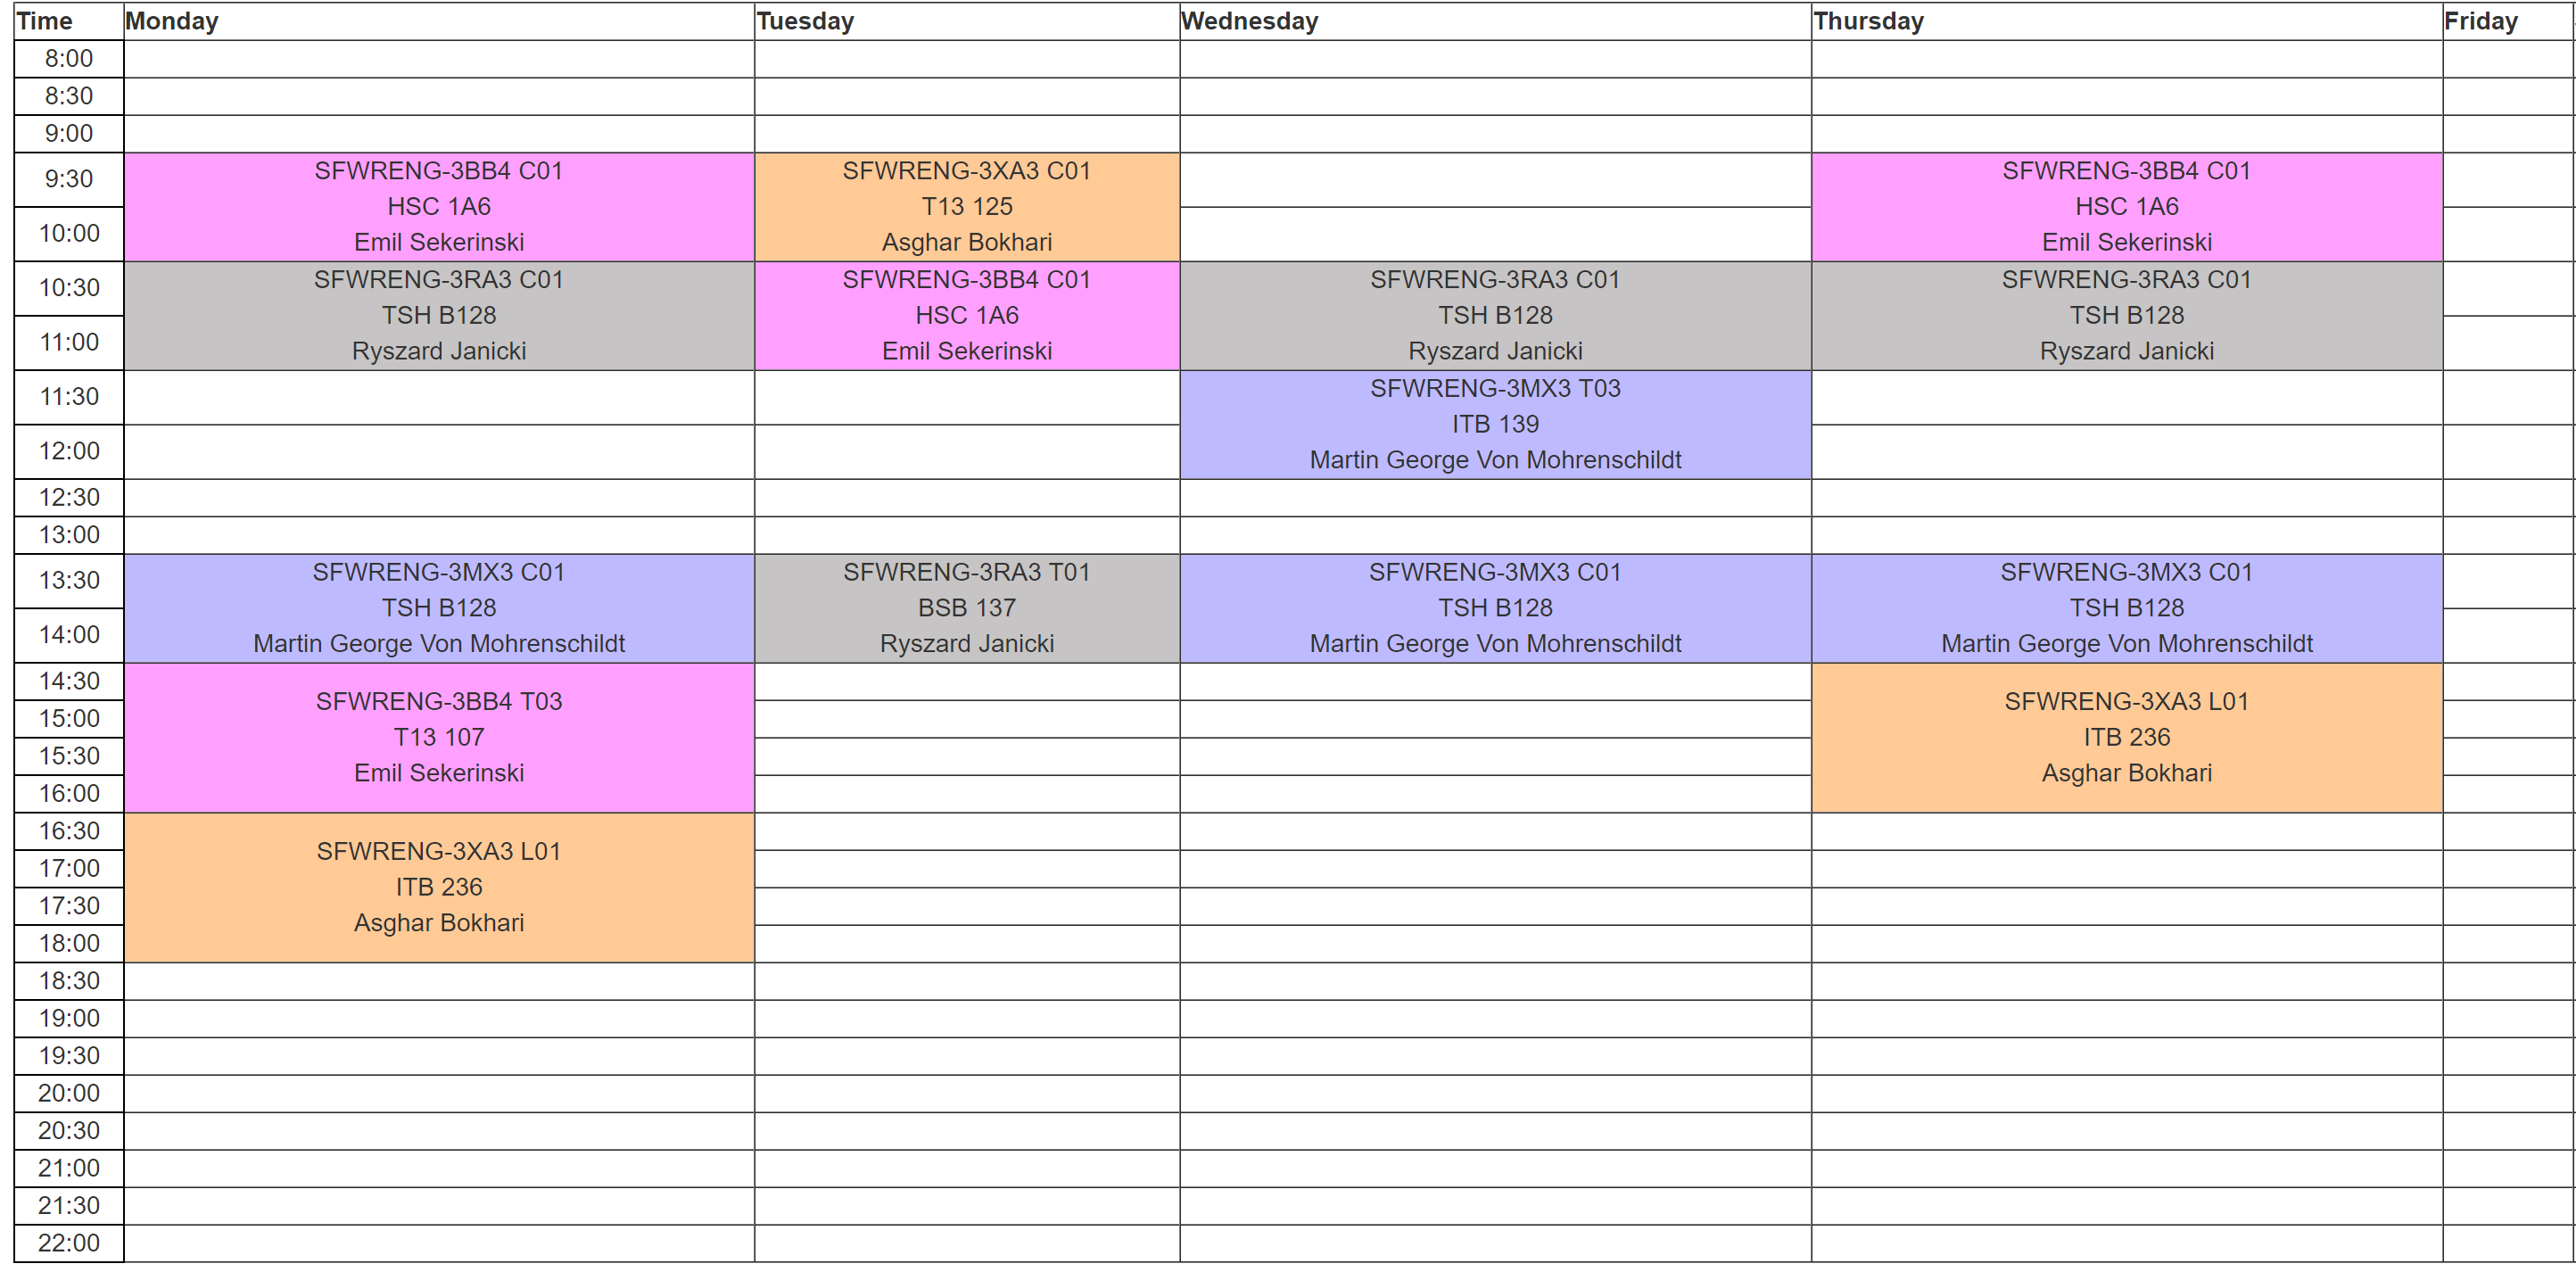
\includegraphics[width=170mm]{Capture.PNG}
    \caption{Example Output}
    \label{fig:my_label}
\end{figure}

\newpage
\section{Non-Functional Requirements}
\textcolor{blue}{
\tab The Non-functional requirements (NFR) of this project describe the appearance and feel of the of the Timetable Generator, as well as requirements such as usability, performance, operational, maintainability, and portability. Underneath each requirement, there is the fit criterion that is used to measure the specific requirement.
}
\subsection{Look and Feel Requirements}
\textcolor{blue}{
\begin{enumerate}
    \item The User-Interface (UI) must be graphical.
    \begin{itemize}
        \item The interface must be entirely made of text-boxes, buttons, graphical lists and tables.
        \item The users must be able to use all the features of the product without the use of a command line terminal.
    \end{itemize}
    \item The UI must be minimal.
    \begin{itemize}
        \item At any given instance, the interface must contain no more than one text-box, two buttons, one graphical list and two tables.
    \end{itemize}
    \item The UI looks professional.
    \begin{itemize}
        \item At least 80\% of the users must agree that the interface is professional.
    \end{itemize}
    \item The UI must look and feel modern.
    \begin{itemize}
        \item At least 80\% of the users must agree that the interface is modern.
    \end{itemize}
    \item The UI must feel responsive.
    \begin{itemize}
        \item For all actions, the results must be displayed no later 500 milliseconds.
    \end{itemize}
\end{enumerate}
}
\subsection{Usability Requirements}
\subsubsection{Ease of use}
\textcolor{blue}{
\begin{enumerate}
    \item The User-Interface (UI) must be minimal.
    \begin{itemize}
        \item At any given instance, the interface must contain no more than one text-box, two buttons, one graphical list and two tables.
    \end{itemize}
    \item The UI must be intuitive.
    \begin{itemize}
        \item Text on all buttons must be self explanatory.
        \item Text on buttons must describe the functions that they perform when they are clicked.
    \end{itemize}
    \item The UI must be clear.
    \begin{itemize}
        \item There must be at least 10 pixels of space between different section of the interface.
        \item The text size must be at least 16pt.
        \item There must be a sharp contrast between texts and their backgrounds.
    \end{itemize}
    \item The UI must be responsive.
    \begin{itemize}
        \item For all actions, the results must be displayed no later 500 milliseconds.
    \end{itemize}
    \item The front-end must minimize as much as possible the number of mouse-clicks that are necessary to generate a timetable after a user enters the website.
    \begin{itemize}
        \item After the users enter their desired courses, only a single click of the generate button must be needed to begin the generation process.
    \end{itemize}
\end{enumerate}
}
\subsubsection{Ease of learning}
\textcolor{blue}{
\begin{enumerate}
    \item There must be visual aids (helpful text, images, animation, etc...) to guide the user.
    \begin{itemize}
        \item There must a written walk-through displayed on the website that can guide the user without any external help.
        \item Text on all buttons must be self explanatory.
        \item Text on buttons must describe the functions that they perform when they are clicked.
        \item There must be text that explain parts of the user interface that are not buttons.
    \end{itemize}
    \item The error messages must be short and easy to understand.
    \begin{itemize}
        \item Messages that explain the errors must be no longer than two sentences each.
        \item The timing conflict error must display the conflicting courses.
    \end{itemize}
\end{enumerate}
}
\subsection{Performance}
\subsubsection{Speed Requirements}
\textcolor{blue}{
\begin{enumerate}
    \item After the user clicks the "Generate" button the generated timetable must be presented to the user in an acceptable time period.
    \begin{itemize}
        \item The generated timetable must be displayed no later 3 seconds.
    \end{itemize}
\end{enumerate}
}
\subsection{Operational and Environmental Requirements}
\subsubsection{Physical Environment}
\textcolor{blue}{
\begin{enumerate}
    \item For this project, there is no specific physical environment in which the product will operate.
\end{enumerate}
}
\subsubsection{Operational Requirements}
\textcolor{blue}{
\begin{enumerate}
    \item The back-end must be compatible with the environment of FireBase since it will hosted there.
    \begin{itemize}
        \item The back-end must be tested in Firebase to make sure that it functions as intended.
    \end{itemize}
    \item The front-end will be operating in users' web-browsers. Therefore, it must be compatible with browser environment.
    \begin{itemize}
        \item The front-end must be tested on Mozilla Firefox, Google Chrome, Opera, Safari, Microsoft Edge and Internet Explorer.
    \end{itemize}
    \item The environment must include a reliable high-bandwidth internet connection in order to be able to server many users concurrently.
    \begin{itemize}
        \item The internet connection must at least be able to download and upload 50 Megabits/second.
    \end{itemize}
\end{enumerate}
}
\subsection{Maintainability and Support Requirements}
\subsubsection{Maintainability Requirements}
\textcolor{blue}{
\begin{enumerate}
    \item The program must be decomposed into a set of small modules that each perform a well-defined set of tasks.
    \begin{itemize}
        \item The developers must use the module pattern.
    \end{itemize}
    \item The source code must be well documented.
    \begin{itemize}
        \item Module interface specification documents must be written and made available for all modules.
        \item Logic behind the code must be explained using comments in the source code explaining the.
    \end{itemize}
    \item The code must follow a standard coding convention.
    \begin{itemize}
        \item All of the source code must conform to the Mozilla coding style.
    \end{itemize}
\end{enumerate}
}
\subsubsection{Support Requirements}
\textcolor{blue}{
\begin{enumerate}
    \item Users must be able report bugs and concerns with the product.
    \begin{itemize}
        \item Users can contact one of the three developers of the product, Sachin, Amit or Mohamed using email.
    \end{itemize}
\end{enumerate}
}
\subsection{Security Requirement}
\textcolor{blue}{
\begin{itemize}
    \item There are no security requirements that apply specifically to this product, seeing as it is hosted online, and no user information is stored.
\end{itemize}
}
\subsection{Cultural Requirements}
\textcolor{blue}{
\begin{itemize}
    \item There are no cultural requirements.
\end{itemize}
}
\subsection{Legal Requirements}
\textcolor{blue}{
\begin{itemize}
    \item There are no legal requirements.
\end{itemize}
}
\subsection{Health and Safety Requirements}
\textcolor{blue}{
\begin{itemize}
    \item There are no health and safety requirements.
\end{itemize}
}
\newpage

\section{Open Issues}

\tab The data that is used in this project is pulled from \url{http://www.timetablegenerator.io}. If the owner of this website decides to modify the format of the data , then this project will have to be re-implemented. 


\section{Off-the-Shelf Solutions}
There are existing similar products, such as \url{http://www.timetablegenerator.io}. The Genzter team has been in contact with the developers of this website, and have received assistance and guidance from them. The data-set can be considered a "ready made component", because this project will be using their data-set (with permission). There are also quite a few open-sourced projects on \url{http://www.github.com} that can be followed.

\section{New Problems}
This project shouldn't create any issues or conflicts with the current implementation environment. As for potential user issues, there should not be any adverse reactions that occur.
\section{Tasks}
The tasks of this project include:
\begin{itemize}
  \item Defining the Problem Statement
  \item Creating the Development Plan
  \item Defining the Requirements
  \item Developing the Proof of Concept
  \item Implementation
  \item Testing
\end{itemize}
This list can change as the development of the project continues.

\section{Risks}
    Some of the main risks of this project are 
    
    \begin{itemize}
        \item 
        Since the data for this website is gathered from \url{https://www.timetablegenerator.io} and if this website gets shutdown, this project won't work. The probability for this being a problem is unlikely. A plan to solve this problem will be to make another program that will parse this data from \url{http://mosaic.mcmaster.ca}.
        \item
        This project will also not work, if the owner of this website decides to make the data private. The probability for this being a problem is also unlikely. A plan to solve this problem will be to make another program that will parse this data from \url{http://mosaic.mcmaster.ca}.
        
    \end{itemize}
\section{Costs}
There should a very small cost associated with this project, seeing as all software used is free, or used under a student license. The cost will come from purchasing the domain and hosting the website. There shouldn't be any other costs associated with the project.
\section{User Documentation}
The only documentation that will be necessary for users are the simple instructions that are on the homepage of the Generator. 



\begin{thebibliography}{9}


 
\end{thebibliography}
\end {document}
